\documentclass[12pt, a4paper]{article}
\usepackage[utf8]{inputenc}
\usepackage[T1]{fontenc}
\usepackage[french]{babel}
\usepackage{graphicx}
\usepackage{hyperref}
\usepackage{geometry}
\usepackage{listings}
\usepackage{xcolor}
\geometry{hmargin=2cm, vmargin=2cm}

\lstdefinelanguage{JSX}{
  keywords={const, let, var, if, else, for, while, return, function, true, false,
            import, export, default, from, async, await, new, try, catch, throw,
            useState, useEffect, null},
  keywordstyle=\color{blue}\bfseries,
  ndkeywords={React, localStorage, window, document, setInterval, clearInterval,
              addEventListener, removeEventListener, parseInt, JSON},
  ndkeywordstyle=\color{teal}\bfseries,
  identifierstyle=\color{black},
  sensitive=true,
  comment=[l]{//},
  morecomment=[s]{/*}{*/},
  commentstyle=\color{green!60!black}\ttfamily,
  stringstyle=\color{red}\ttfamily,
  morestring=[b]',
  morestring=[b]"
}

\lstset{
    language=JSX,
    backgroundcolor=\color{black!5},
    basicstyle=\ttfamily\footnotesize,
    keywordstyle=\color{blue}\bfseries,
    stringstyle=\color{red},
    commentstyle=\color{green!60!black},
    numbers=left,
    numberstyle=\tiny\color{gray},
    stepnumber=1,
    numbersep=8pt,
    showstringspaces=false,
    breaklines=true,
    frame=single,
    extendedchars=true,
    literate=
      {é}{{\'{e}}}1
      {è}{{\`{e}}}1
      {ê}{{\^{e}}}1
      {à}{{\`{a}}}1
      {â}{{\^{a}}}1
      {î}{{\^{i}}}1
      {ô}{{\^{o}}}1
      {û}{{\^{u}}}1
      {ù}{{\`{u}}}1
      {ç}{{\c{c}}}1
      {'}{{'}}1
      {→}{{->}}1
}

\title{\textbf{Compte-rendu du TP 5 : React Moderne, JSX \& Les Hooks Fondamentaux\\(useState \& useEffect)}}
\author{
    Réalisé par : \textbf{JOSEPH MUKUBU KAPOYA} \\
    \textit{5ème Datascience et IA, Groupe 1}
}
\date{\today}

\begin{document}
\maketitle

\section*{Introduction}
Ce cinquième atelier pratique marque l'entrée dans l'univers \textbf{React} — la bibliothèque d'interface utilisateur au cœur de la stack MERN. Nous construisons de A à Z un \textbf{compteur interactif} complet qui exploite les deux hooks fondamentaux :
\begin{itemize}
    \item \texttt{useState} : pour gérer l'état réactif (valeur, pas, historique, total clics).
    \item \texttt{useEffect} : pour les effets de bord (titre onglet, persistence localStorage, chronomètre, clavier).
\end{itemize}
Les trois défis pratiques implémentent les fonctionnalités avancées : bornes limites, sauvegarde de l'historique et contrôle au clavier avec nettoyage propre.

\section{Réponses aux Encadrés « Prédisez »}

\subsection*{Prédisez 1 : Variable ordinaire vs useState}
\textbf{Question :} Si on clique sur +1, le \texttt{console.log} affiche 1, 2, 3... Mais qu'affiche le \texttt{<p>} à l'écran ? Pourquoi reste-t-il à 0 ?

\textbf{Réponse :} Le paragraphe \texttt{<p>} reste désespérément bloqué à \textbf{0}. Une variable \texttt{let} ordinaire est une donnée \textit{privée} de la fonction composant. Lorsque sa valeur change en mémoire, \textbf{React n'est pas notifié}. Aucun re-rendu n'est déclenché, donc le DOM reste figé. Seul le \texttt{Hook useState} — via son setter \texttt{setValeur()} — signale à React qu'une donnée a changé et que la fonction composant doit être réexécutée pour mettre à jour l'affichage.

\subsection*{Prédisez 2 : Persistance localStorage et F5}
\textbf{Question :} Que se passe-t-il si vous modifiez la valeur à 42 puis appuyez sur F5 ?

\textbf{Réponse :} Le compteur \textbf{ne revient pas à zéro}. Grâce à l'initialisation paresseuse du \texttt{useState} :
\begin{lstlisting}
const [count, setCount] = useState(() => {
  const sauvegarde = localStorage.getItem('mon_compteur_valeur');
  return sauvegarde !== null ? parseInt(sauvegarde, 10) : 0;
});
\end{lstlisting}
et à l'effet de bord qui sauvegarde en temps réel :
\begin{lstlisting}
useEffect(() => {
  localStorage.setItem('mon_compteur_valeur', count.toString());
}, [count]);
\end{lstlisting}
Au rechargement de la page, React lit immédiatement la valeur \texttt{"42"} depuis le \texttt{localStorage} et l'affiche directement — sans passer par zéro.

\section{Captures d'Écran de l'Application}

\subsection{État initial de l'application}

\begin{figure}[htbp]
    \centering
    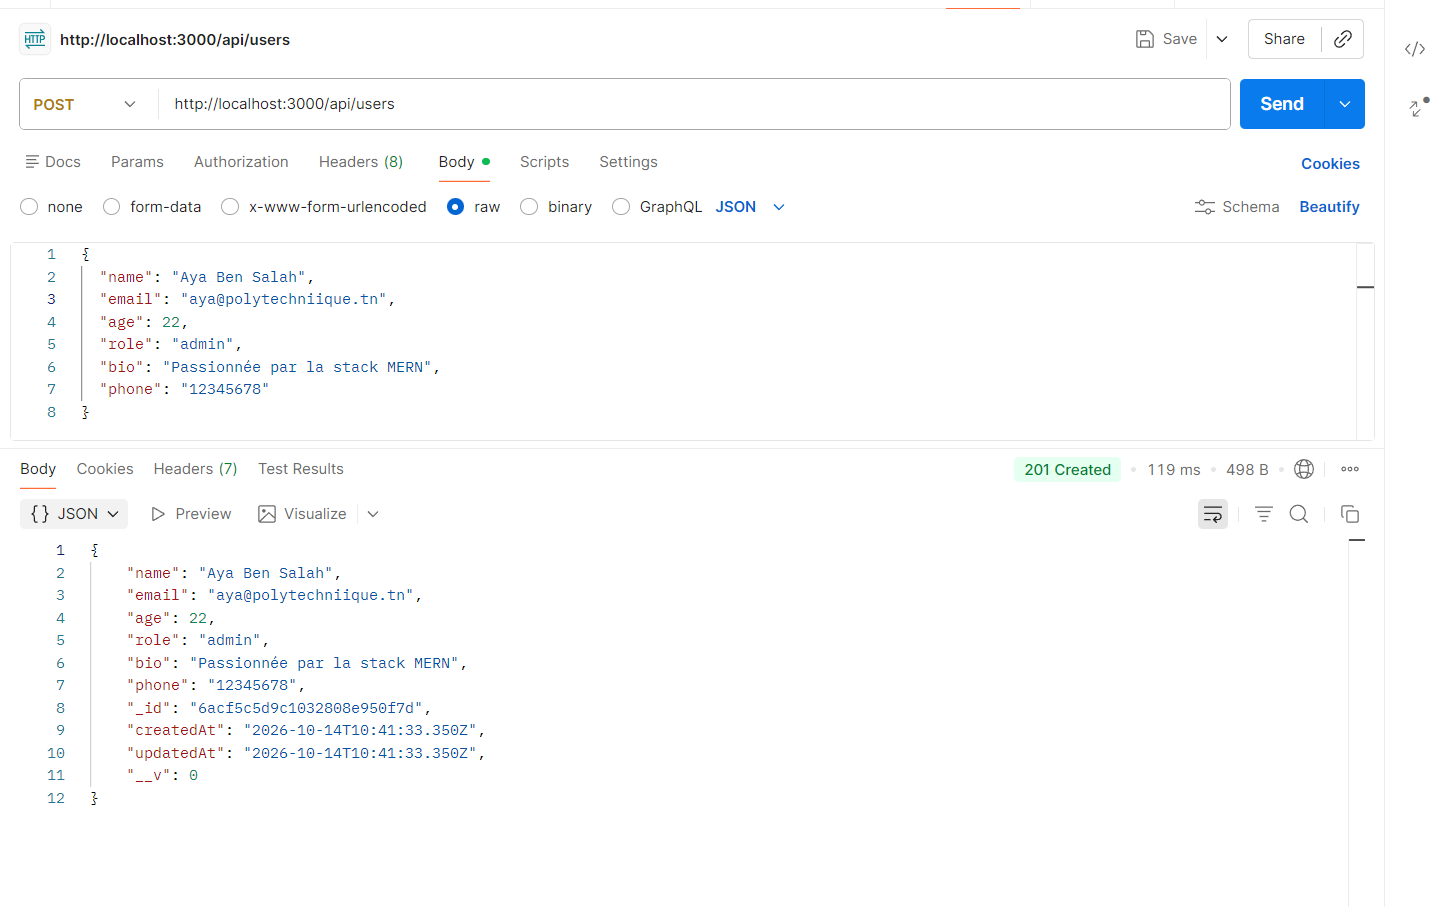
\includegraphics[width=0.78\textwidth]{reactTP5-1.png}
    \caption{Application au chargement initial -- compteur à 0, timer en cours}
    \vspace{0.1cm}
    \small \textit{Description :} Vue complète de l'application au démarrage : le \textbf{Header} affiche le titre et la date du jour en français via \texttt{toLocaleDateString('fr-FR')}. Le compteur affiche \textbf{0} (gris neutre). Le message d'historique indique "Aucun clic pour le moment". Le chronomètre \textbf{AutoTimer} tourne depuis le montage.
\end{figure}

\clearpage
\subsection{Compteur positif après 3 clics avec pas de 5}

\begin{figure}[htbp]
    \centering
    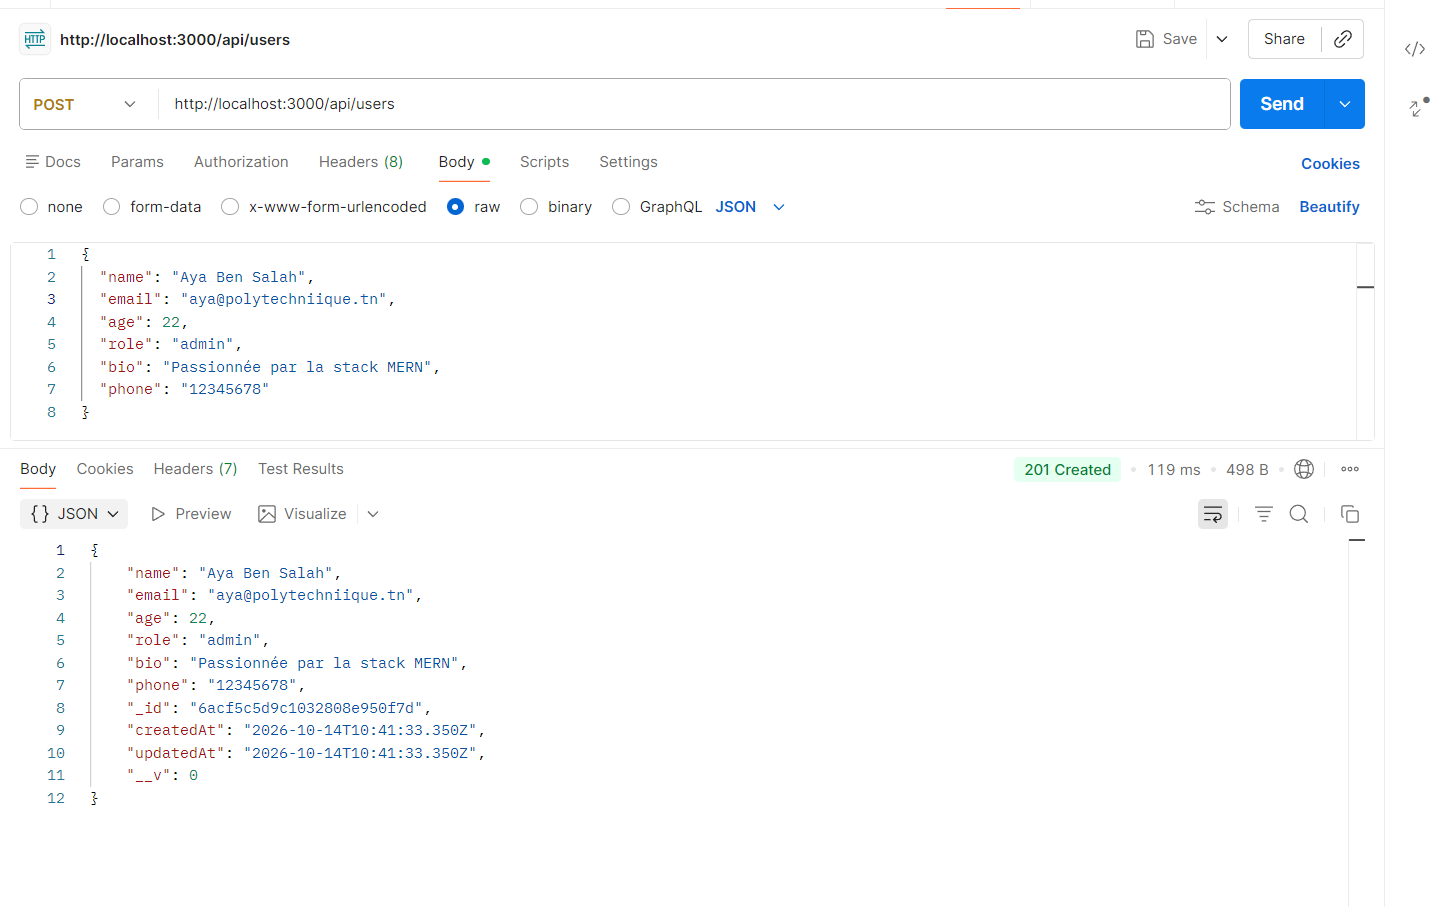
\includegraphics[width=0.78\textwidth]{reactTP5-2.png}
    \caption{Après 3 clics sur +5 -- compteur à 15, affiché en vert}
    \vspace{0.1cm}
    \small \textit{Description :} Après sélection du pas 5 et 3 clics sur "+5" : le compteur affiche \textbf{+15 en vert} (classe \texttt{positive}), la dernière action indique "Ajout de 5", le total des clics est 3, l'historique affiche \texttt{+5, +5, +5}. L'onglet du navigateur affiche "Compteur : 15".
\end{figure}

\clearpage
\subsection{Défi 1 : Alerte seuil maximal atteint}

\begin{figure}[htbp]
    \centering
    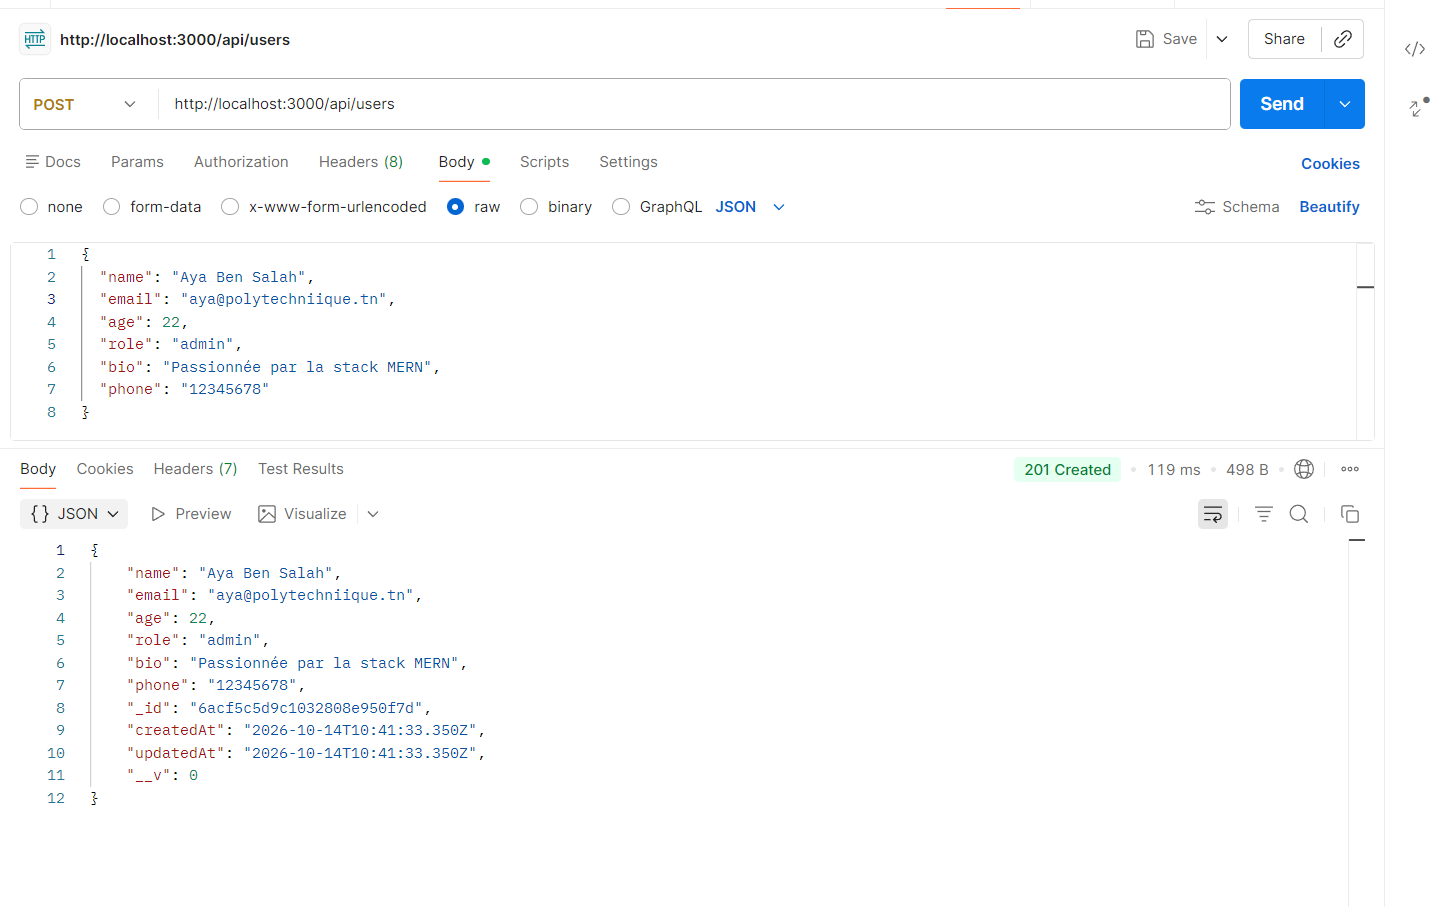
\includegraphics[width=0.78\textwidth]{reactTP5-3.png}
    \caption{Défi 1 -- Seuil maximal de 50 atteint, bouton désactivé}
    \vspace{0.1cm}
    \small \textit{Description :} Lorsque le compteur atteint \textbf{50} (borne maximale), le bouton \texttt{+} est désactivé (\texttt{disabled}) et le message d'alerte "\textbf{Seuil maximal de 50 atteint !}" s'affiche en violet. Même logique pour la borne inférieure \textbf{-50}.
\end{figure}

\clearpage
\subsection{Défi 2 : Persistance de l'historique après F5}

\begin{figure}[htbp]
    \centering
    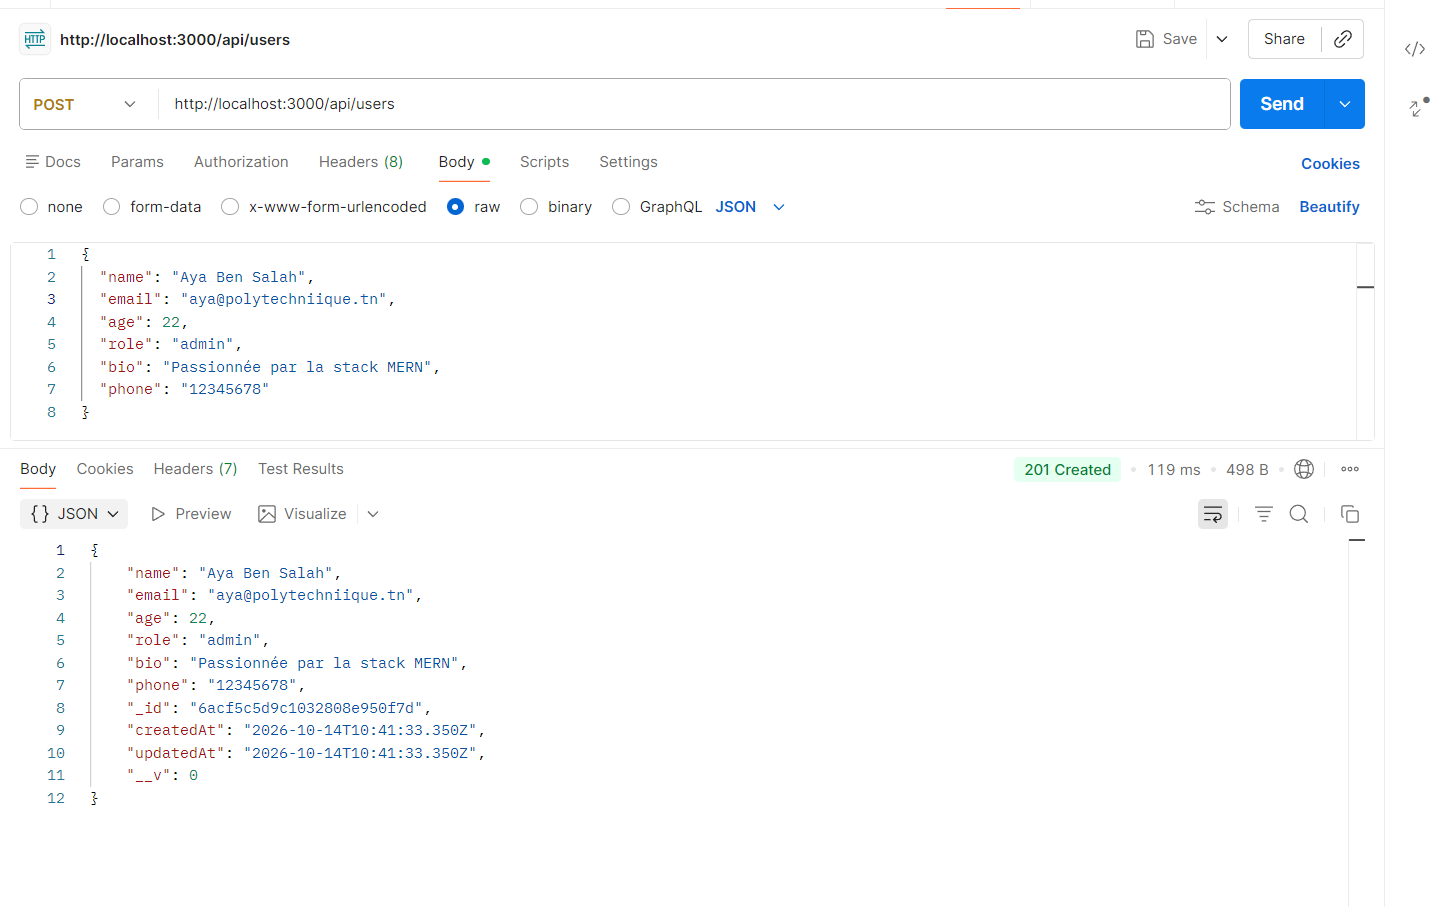
\includegraphics[width=0.78\textwidth]{reactTP5-4.png}
    \caption{Défi 2 -- LocalStorage avec valeur et historique restaurés après rechargement}
    \vspace{0.1cm}
    \small \textit{Description :} Vue des DevTools (F12 → Application → Local Storage) montrant les deux clés sauvegardées : \texttt{mon\_compteur\_valeur} et \texttt{mon\_compteur\_historique} (JSON sérialisé). Après F5, la valeur du compteur \textbf{et} l'historique complet sont restaurés.
\end{figure}

\clearpage
\subsection{Chronomètre AutoTimer et contrôle Pause/Reprendre}

\begin{figure}[htbp]
    \centering
    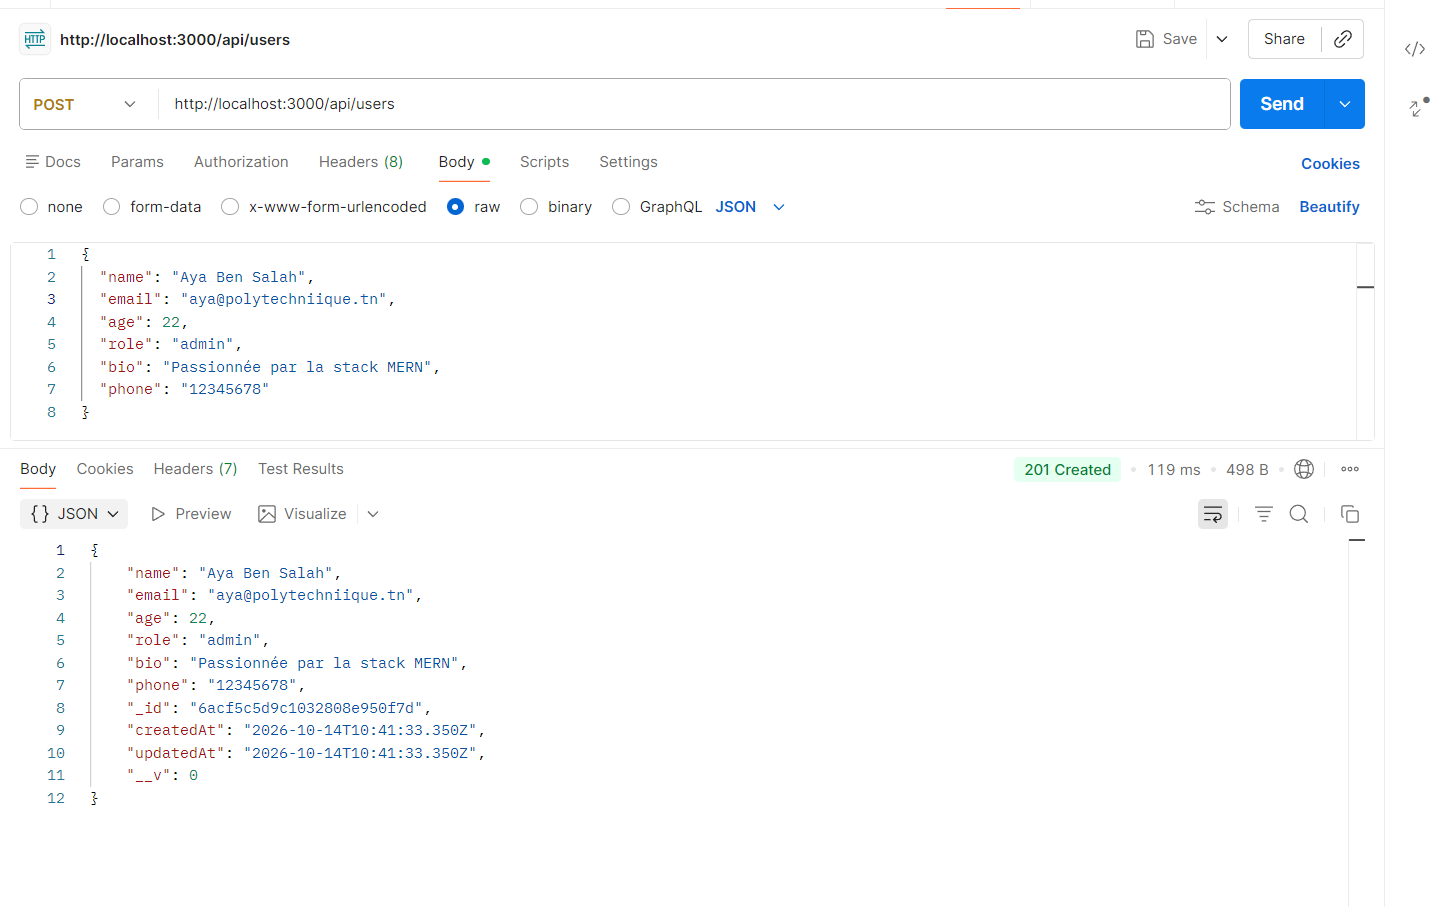
\includegraphics[width=0.78\textwidth]{reactTP5-5.png}
    \caption{AutoTimer en cours -- contrôle Pause/Reprendre et nettoyage useEffect}
    \vspace{0.1cm}
    \small \textit{Description :} Le composant \textbf{AutoTimer} affiche les secondes écoulées. Le bouton "Pause" arrête proprement le \texttt{setInterval} via la fonction de nettoyage \texttt{return () => clearInterval(intervalId)}. Le bouton "Masquer le Chronomètre" démonte le composant sans fuite mémoire.
\end{figure}

\newpage
\section{Code Source Intégral du Projet}

\subsection{Composant Header : \texttt{src/components/Header.jsx}}
\begin{lstlisting}
import React from 'react';

export default function Header({ titre, sousTitre }) {
  // Logique JavaScript : formatage de la date locale
  const dateDuJour = new Date().toLocaleDateString('fr-FR', {
    weekday: 'long', year: 'numeric', month: 'long', day: 'numeric',
  });

  return (
    <header className="header">
      <h1>{titre}</h1>
      <p>{sousTitre}</p>
      <small style={{ color: '#94a3b8', display: 'block', marginTop: '6px' }}>
        Date de la session : {dateDuJour}
      </small>
    </header>
  );
}
\end{lstlisting}

\subsection{Composant Counter complet (avec les 3 Défis) : \texttt{src/components/Counter.jsx}}
\begin{lstlisting}
import React, { useState, useEffect } from 'react';

const MIN = -50;  // Defi 1 : borne minimale
const MAX = 50;   // Defi 1 : borne maximale

export default function Counter() {
  // Initialisation depuis localStorage (Etape 5)
  const [count, setCount] = useState(() => {
    const sauvegarde = localStorage.getItem('mon_compteur_valeur');
    return sauvegarde !== null ? parseInt(sauvegarde, 10) : 0;
  });
  const [step, setStep] = useState(1);
  const [message, setMessage] = useState('Aucun clic pour le moment');
  const [totalClics, setTotalClics] = useState(0);

  // Defi 2 : restauration historique
  const [historique, setHistorique] = useState(() => {
    const sauvegarde = localStorage.getItem('mon_compteur_historique');
    return sauvegarde ? JSON.parse(sauvegarde) : [];
  });
  const [alerteMax, setAlerteMax] = useState('');

  // EFFET A : Titre de l'onglet
  useEffect(() => { document.title = 'Compteur : ' + count; }, [count]);

  // EFFET B : Sauvegarde valeur
  useEffect(() => {
    localStorage.setItem('mon_compteur_valeur', count.toString());
  }, [count]);

  // Defi 2 : Sauvegarde historique (JSON.stringify obligatoire pour tableau)
  useEffect(() => {
    localStorage.setItem('mon_compteur_historique', JSON.stringify(historique));
  }, [historique]);

  // Defi 3 : Controle au clavier avec NETTOYAGE OBLIGATOIRE
  useEffect(() => {
    const handleKeyDown = (e) => {
      if (e.key === 'ArrowUp') {
        setCount((prev) => {
          if (prev + step > MAX) { setAlerteMax(`Seuil maximal atteint !`); return prev; }
          setAlerteMax('');
          setMessage('Ajout de ' + step + ' (clavier)');
          setTotalClics((t) => t + 1);
          setHistorique((h) => [...h, '+' + step]);
          return prev + step;
        });
      } else if (e.key === 'ArrowDown') {
        setCount((prev) => {
          if (prev - step < MIN) { setAlerteMax(`Seuil minimal atteint !`); return prev; }
          setAlerteMax('');
          setMessage('Retrait de ' + step + ' (clavier)');
          setTotalClics((t) => t + 1);
          setHistorique((h) => [...h, '-' + step]);
          return prev - step;
        });
      }
    };
    window.addEventListener('keydown', handleKeyDown);
    // IMPERATIF : detachement de l'ecouteur pour eviter fuite memoire
    return () => { window.removeEventListener('keydown', handleKeyDown); };
  }, [step]);

  const handleIncrement = () => {
    if (count + step > MAX) { setAlerteMax(`Seuil maximal de ${MAX} atteint !`); return; }
    setAlerteMax('');
    setCount(count + step);
    setMessage('Ajout de ' + step);
    setTotalClics(totalClics + 1);
    setHistorique([...historique, '+' + step]);
  };

  const handleDecrement = () => {
    if (count - step < MIN) { setAlerteMax(`Seuil minimal de ${MIN} atteint !`); return; }
    setAlerteMax('');
    setCount(count - step);
    setMessage('Retrait de ' + step);
    setTotalClics(totalClics + 1);
    setHistorique([...historique, '-' + step]);
  };

  const handleReset = () => {
    setCount(0); setMessage('Remise a zero');
    setTotalClics(totalClics + 1); setHistorique([]); setAlerteMax('');
  };

  const getStyleClass = () => {
    if (count > 0) return 'counter-display positive';
    if (count < 0) return 'counter-display negative';
    return 'counter-display zero';
  };

  return (
    <div className="counter-card">
      <div className={getStyleClass()}>{count}</div>
      {alerteMax && <p className="alerte">{alerteMax}</p>}
      <div className="btn-group">
        <button className="btn btn-dec" onClick={handleDecrement}
          disabled={count - step < MIN}>-{step}</button>
        <button className="btn btn-reset" onClick={handleReset}>Reset</button>
        <button className="btn btn-inc" onClick={handleIncrement}
          disabled={count + step > MAX}>+{step}</button>
      </div>
      <div className="step-control">
        <label>Pas : </label>
        <select value={step} onChange={(e) => setStep(parseInt(e.target.value, 10))}>
          <option value="1">1</option>
          <option value="2">2</option>
          <option value="5">5</option>
          <option value="10">10</option>
        </select>
      </div>
      <div className="history-card">
        <p><strong>Derniere action : </strong>{message}</p>
        <p><strong>Total des clics : </strong>{totalClics}</p>
        {historique.length > 0 && (
          <p><strong>Historique : </strong>{historique.join(', ')}</p>
        )}
        <p className="hint">Utilisez les fleches haut/bas pour piloter au clavier</p>
      </div>
    </div>
  );
}
\end{lstlisting}

\subsection{Composant AutoTimer avec nettoyage : \texttt{src/components/AutoTimer.jsx}}
\begin{lstlisting}
import React, { useState, useEffect } from 'react';

export default function AutoTimer() {
  const [seconds, setSeconds] = useState(0);
  const [isRunning, setIsRunning] = useState(true);

  useEffect(() => {
    let intervalId = null;
    if (isRunning) {
      intervalId = setInterval(() => {
        setSeconds((prev) => prev + 1);
      }, 1000);
    }
    // NETTOYAGE : evite la fuite memoire lors du demontage ou quand isRunning change
    return () => { if (intervalId) clearInterval(intervalId); };
  }, [isRunning]);

  return (
    <div className="timer-box">
      <span>Chronometre : <strong>{seconds}s</strong></span>
      <button className="btn" onClick={() => setIsRunning(!isRunning)}>
        {isRunning ? 'Pause' : 'Reprendre'}
      </button>
    </div>
  );
}
\end{lstlisting}

\subsection{Composant racine : \texttt{src/App.jsx}}
\begin{lstlisting}
import React, { useState } from 'react';
import Header from './components/Header';
import Counter from './components/Counter';
import AutoTimer from './components/AutoTimer';
import './index.css';

export default function App() {
  const [showTimer, setShowTimer] = useState(true);

  return (
    <div className="app-container">
      <Header
        titre="Mon Super Compteur React"
        sousTitre="Maitrise des Hooks fondamentaux useState et useEffect"
      />
      <Counter />
      <div style={{ textAlign: 'center', margin: '1rem 0' }}>
        <button className="btn btn-reset" onClick={() => setShowTimer(!showTimer)}>
          {showTimer ? 'Masquer le Chronometre' : 'Afficher le Chronometre'}
        </button>
      </div>
      {showTimer && <AutoTimer />}
    </div>
  );
}
\end{lstlisting}

\section*{Conclusion}
Ce TP 5 valide les fondamentaux de React pour la stack MERN. Le Hook \texttt{useState} confère de la \textbf{mémoire réactive} aux composants : chaque appel au setter déclenche un re-rendu chirurgical. Le Hook \texttt{useEffect} synchronise le composant avec le monde extérieur (DOM, API, timers) en contrôlant précisément \textbf{quand} et \textbf{combien de fois} l'effet s'exécute grâce au tableau de dépendances. La fonction de nettoyage garantit qu'aucune fuite mémoire ne survient lors du démontage. L'application résultante — compteur avec bornes, historique persisté et contrôle clavier — illustre concrètement ces principes sur une interface réelle.

\end{document}
